\section{Results}
\subsection{Plaquette expectation value}
As first comparison and confirmation of the presented setup, the plaquette expectation value are of interest. It is defined as the following:
\begin{align}
	\Braket{P} = \Braket{\sum_{\vec{r}}\frac{P_{\vec{r}}+P_{\vec{r}}^{\dag}}{2}}.
\end{align}
From the scaling of the Hamiltonian in respect to $g$, $\lim_{g\rightarrow\infty}\Braket{P}=0$ and $\lim_{g\rightarrow0}\Braket{P}=1$ are expected.
% TODO: what does the exp value mean intuitivly? (percentage contribution to the hamiltonian) 
This behaviour is intuitive, when thinking of the plaquette expectation value as a measure of the contribution from the plaquette operator to the Hamiltonian. Since the electric Hamiltonian is proportional to $g^2$, it should dominate for strong couplings. For weak couplings, the magnetic Hamiltonian is expected to dominate, and thus the plaquette operator, since it is proportional to $1/g^2$. When comparing this expectation to the following results, one has always to be mindful of the fact, that the x-axis shows $\beta=1/g^2$.

\Cref{fig:2exp} is the result of the calculation, confirming the expected.
\begin{figure}[h]
	\begin{center}
		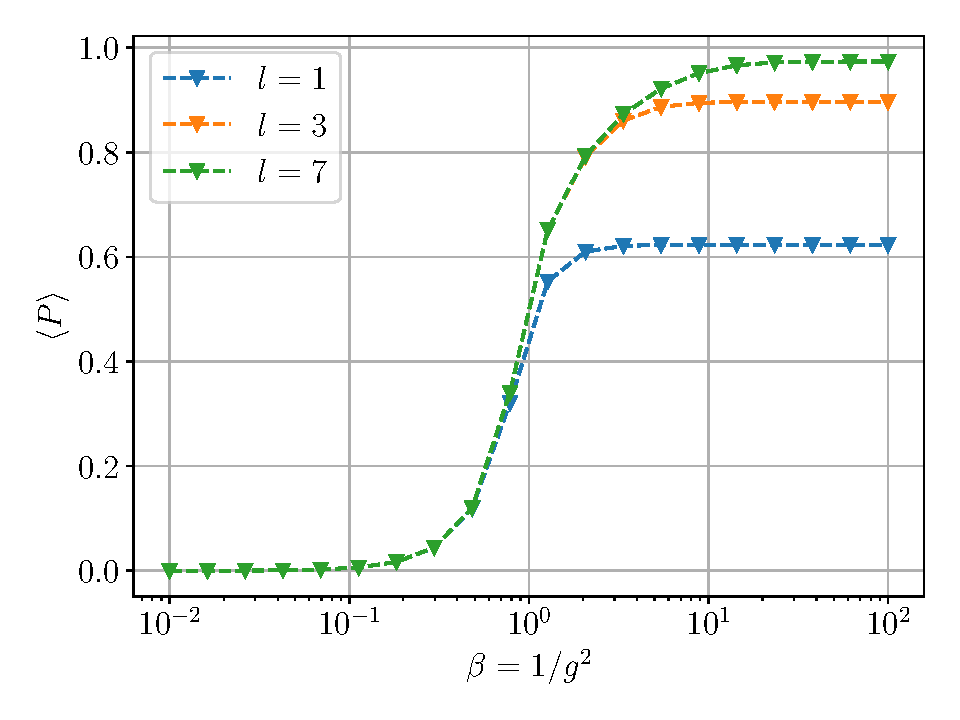
\includegraphics[width=0.45\textwidth]{images/PlaquetteExp2x2PBC.pdf}
	\end{center}
	\caption{plaquette expectation values for a $2\cross2$ lattice with PBC.}\label{fig:2exp}
\end{figure}
An interesting but not surprising observation is the convergence of the expectation value to 1 for large $\beta$ with the order of truncation. This is due to the approach to continuum theory for large truncations. Thus using large $l$ is favourable.

As a next step, larger lattices of dimensions $3\cross3$ are calculated. \Cref{fig:3exp} shows the results. The linear scale and range of $\beta$ is chosen, to be comparable to fig. 5 from Arianna Crippa et al. (2024)\cite{crippa2024}.
\begin{figure}[h]
	\begin{center}
		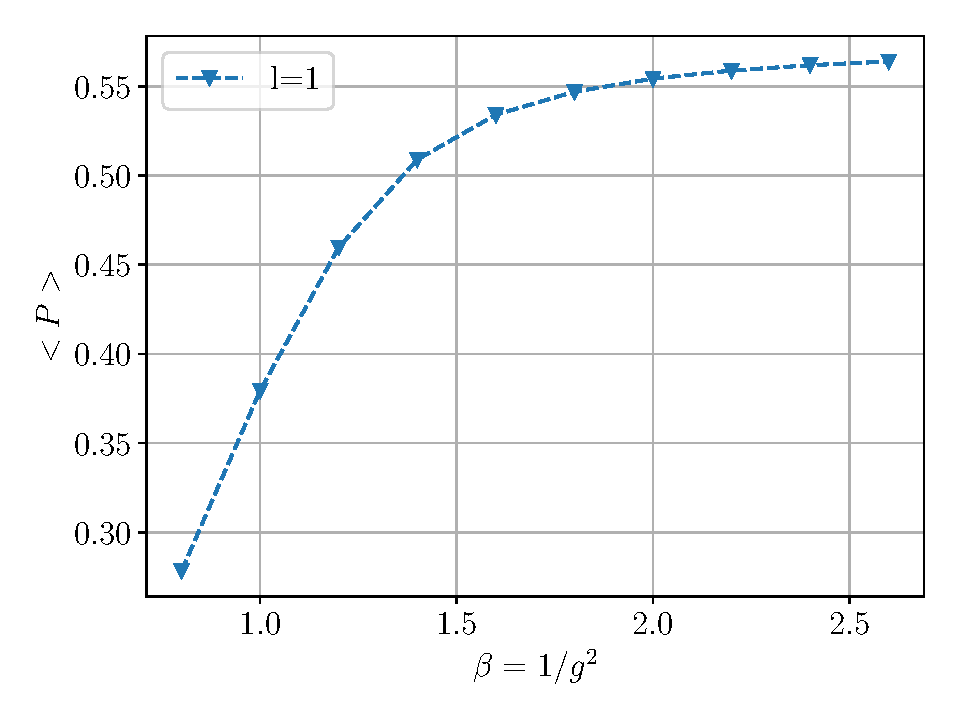
\includegraphics[width=0.45\textwidth]{images/PlaquetteExp3x3PBC.pdf}
	\end{center}
	\caption{Plaquette expectation values for a $3\cross3$ lattice with PBC.}\label{fig:3exp}
\end{figure}
\newpage
It again confirms the convergence to 1 with increasing $\beta$ and weakening truncation. Weak truncation meaning larger $l$, since for infinite $l$ the truncation effect would vanish.


\subsection{Quark-Antiquark potential}
Now for calculating the quark antiquark potential, the energy of the chargeless lattice $\hat{H}_{0}$ is subtracted:
\begin{align}
  V = \Braket{\hat{H}} - \Braket{\hat{H}_{0}}
\end{align}
with $\hat{H}$ being the lattice with the desired charge. This reduces the total energy to the potential energy emitted by the charge and renormalizes it when approaching continuum theory. % TODO: correct?
For the purpose of this work, one charge is being placed in the bottom left corner and the opposite charge at a lattice site with desired distance.
The study of the effect of different setups on charge pairs with the same distance is also of interest. Thus the truncation $l$ is varied from 1 to 3 and compared to the original $3 \cross 3$ lattice with no PBC, with PBC and a lattice with dimensions $4\cross 4$. With these different setups \Cref{fig:qqbar} is obtained. Throughout this section this is the central Figure, that is discussed.
\begin{figure}[h]
	\begin{center}
		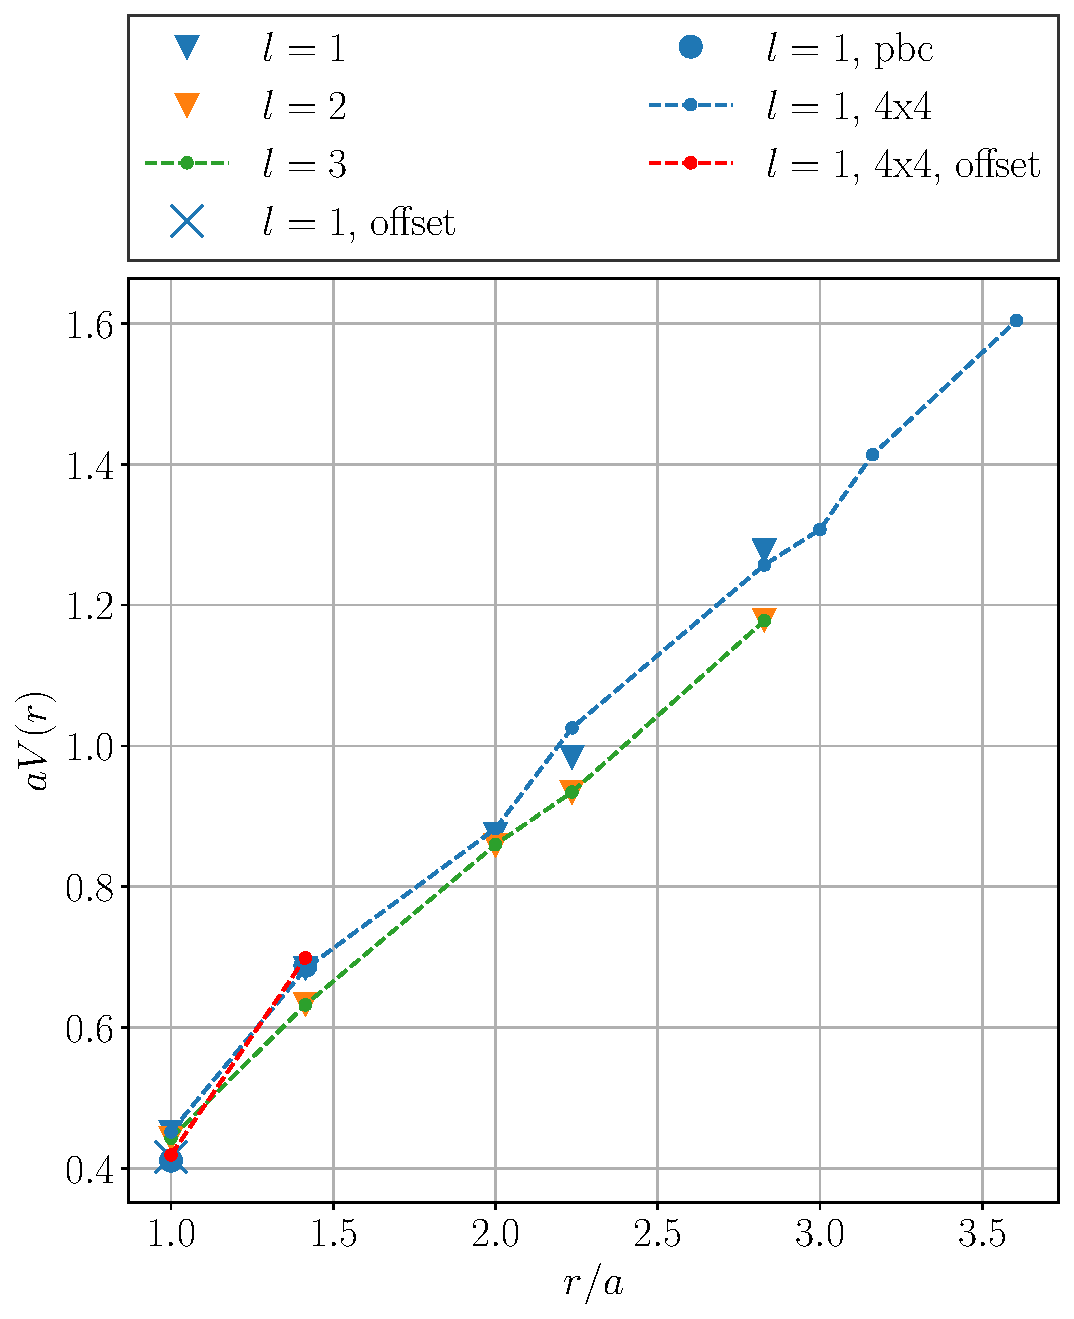
\includegraphics[width=0.45\textwidth]{images/quark_antiquark_potential_g_1.pdf}
	\end{center}
	\caption{Quark-Antiquark potential for different but comparable setups at $g=\num{1}$. By default $3\cross3$ dimensions and no PBC, if not stated otherwise.}\label{fig:qqbar}
\end{figure}

The most basic setup is a $3\cross 3$ lattice with no PBC and a truncation of $l=1$. The potential raises linearly with increasing distance
\begin{align}
	V(r) = \sigma r,
\end{align}
where $\sigma$ is the so called string tension.
From a classical perspective this is surprising. But this phenomena has already been reviewed \cite{RevModPhys.51.659} and it is indeed confinement.
%TODO: More explanation

Now different lattice parameters are varied.
Starting with a different truncation $l$, here 2 and 3, the potential has the same behaviour, but is more linear. This shows, that indeed the truncation effects vanish when choosing a weaker truncation, i.e. large $l$. Already choosing a truncation of $l=2$ is a significant improvement. Furthermore improvement with $l=3$ is marginal.

For the next comparison, the charge pair is not set at the rim, but at the center. The scene is sketched in \Cref{fig:3x3no}. The continuum theory has translational invariance. Since moving the charge pair away from the rim gives approximate translational invariance, the lattice converges to the continuum theory. The normal setup is used for our initial calculation with $l=1$ at $r=1$ (upside down triangle). The potential of the offset setup is now depicted by the blue cross in \Cref{fig:qqbar}. Unfortunately the lattice is too small, such that no other distances are really feasible. Thus there is no real comparison possible.
\begin{figure}[h]
	\begin{center}
		
\subfloat[normal]{
	\begin{tikzpicture}[thick,decoration={
					markings,
					mark=at position 0.5 with {\arrow{>}}}
		]

		\tikzset{
			site/.style={
					circle, draw=gray, fill=gray!20, line width=1.5pt, inner sep=0pt, outer sep=4pt, minimum size=0.4cm
				},
			pcharge/.style={
					circle, draw=red, fill=red!20, line width=1.5pt, inner sep=0pt, outer sep=4pt, minimum size=0.4cm
				},
			ncharge/.style={
					circle, draw=blue, fill=blue!20, line width=1.5pt, inner sep=0pt, outer sep=4pt, minimum size=0.4cm
				},
		}
		\node[pcharge](s1){\textbf{$+$}};
		\node[site, right=0.8cm of s1](s2){};
		\node[site, right=0.8cm of s2](s3){};
		\node[ncharge, above=0.8cm of s1](s4){\textbf{-}};
		\node[site, above=0.8cm of s2](s5){};
		\node[site, above=0.8cm of s3](s6){};
		\node[site, above=0.8cm of s4](s7){};
		\node[site, above=0.8cm of s5](s8){};
		\node[site, above=0.8cm of s6](s9){};


		\draw[postaction={decorate}] (s1)--(s2);
		\draw[postaction={decorate}] (s2)--(s3);

		\draw[postaction={decorate}] (s1)--(s4);
		\draw[postaction={decorate}] (s2)--(s5);
		\draw[postaction={decorate}] (s3)--(s6);

		\draw[postaction={decorate}] (s4)--(s5);
		\draw[postaction={decorate}] (s5)--(s6);

		\draw[postaction={decorate}] (s4)--(s7);
		\draw[postaction={decorate}] (s5)--(s8);
		\draw[postaction={decorate}] (s6)--(s9);

		\draw[postaction={decorate}] (s7)--(s8);
		\draw[postaction={decorate}] (s8)--(s9);

	\end{tikzpicture}
}
\hspace{0.01\textwidth}
\subfloat[offset]{
	\begin{tikzpicture}[thick,decoration={
					markings,
					mark=at position 0.5 with {\arrow{>}}}
		]

		\tikzset{
			site/.style={
					circle, draw=gray, fill=gray!20, line width=1.5pt, inner sep=0pt, outer sep=4pt, minimum size=0.4cm
				},
			pcharge/.style={
					circle, draw=red, fill=red!20, line width=1.5pt, inner sep=0pt, outer sep=4pt, minimum size=0.4cm
				},
			ncharge/.style={
					circle, draw=blue, fill=blue!20, line width=1.5pt, inner sep=0pt, outer sep=4pt, minimum size=0.4cm
				},
		}
		\node[site](s1){};
		\node[pcharge, right=0.8cm of s1](s2){\textbf{$+$}};
		\node[site, right=0.8cm of s2](s3){};
		\node[site, above=0.8cm of s1](s4){};
		\node[ncharge, above=0.8cm of s2](s5){\textbf{-}};
		\node[site, above=0.8cm of s3](s6){};
		\node[site, above=0.8cm of s4](s7){};
		\node[site, above=0.8cm of s5](s8){};
		\node[site, above=0.8cm of s6](s9){};


		\draw[postaction={decorate}] (s1)--(s2);
		\draw[postaction={decorate}] (s2)--(s3);

		\draw[postaction={decorate}] (s1)--(s4);
		\draw[postaction={decorate}] (s2)--(s5);
		\draw[postaction={decorate}] (s3)--(s6);

		\draw[postaction={decorate}] (s4)--(s5);
		\draw[postaction={decorate}] (s5)--(s6);

		\draw[postaction={decorate}] (s4)--(s7);
		\draw[postaction={decorate}] (s5)--(s8);
		\draw[postaction={decorate}] (s6)--(s9);

		\draw[postaction={decorate}] (s7)--(s8);
		\draw[postaction={decorate}] (s8)--(s9);

	\end{tikzpicture}
}

		\caption{$3\cross 3$ lattice with two charge pairs of same distance but different position.}\label{fig:3x3no}
	\end{center}
\end{figure}

A clever way to avoid rims, is to use periodic boundary conditions (PBC). The disadvantage is that the shortest path is not always the path through the center links, but through the links that are introduced by the PBC. This limits our possible charge pair setups, since already for a $3 \cross 3$ lattice with PBC, there are only two different setups. All other setups can be created by translation and rotation of those two. They are depicted in \Cref{fig:3x3pbcv1}
Since there is translational invariance, the continuum theory should be approached. Even though it is translational invariance, it is not the same as in the continuum limit, since with PBC the paths also loop around. Those paths are also colored in \Cref{fig:3x3pbcv1}. This should again introduce lattice fragments.
The resulting potentials are marked with circles in \Cref{fig:qqbar}. There is no real influence to be seen.
\begin{figure}[h]
	\begin{center}
		\subfloat[]{
			\scalebox{0.7}{
				
\begin{tikzpicture}[thick,decoration={
				markings,
				mark=at position 0.5 with {\arrow{>}}}
	]

	\tikzset{
		site/.style={
				circle, draw=gray, fill=gray!20, line width=1.5pt, inner sep=0pt, outer sep=4pt, minimum size=0.4cm
			},
		pcharge/.style={
				circle, draw=red, fill=red!20, line width=1.5pt, inner sep=0pt, outer sep=4pt, minimum size=0.4cm
			},
		ncharge/.style={
				circle, draw=blue, fill=blue!20, line width=1.5pt, inner sep=0pt, outer sep=4pt, minimum size=0.4cm
			},
	}
	\node[site](s1){};
	\node[site, right=0.8cm of s1](s2){};
	\node[site, right=0.8cm of s2](s3){};
	\node[site, above=0.8cm of s1](s4){};
	\node[pcharge, above=0.8cm of s2](s5){\textbf{$+$}};
	\node[site, above=0.8cm of s3](s6){};
	\node[site, above=0.8cm of s4](s7){};
	\node[ncharge, above=0.8cm of s5](s8){\textbf{-}};
	\node[site, above=0.8cm of s6](s9){};

	\node[above=0.8cm of s7](c1){};
	\node[above=0.8cm of s8](c2){};
	\node[above=0.8cm of s9](c3){};

	\node[right=0.8cm of s3](c4){};
	\node[right=0.8cm of s6](c5){};
	\node[right=0.8cm of s9](c6){};


	\draw[postaction={decorate}] (s1)--(s2);
	\draw[postaction={decorate}] (s2)--(s3);

	\draw[postaction={decorate}] (s1)--(s4);
	\draw[postaction={decorate}, draw=Dandelion] (s2)--(s5);
	\draw[postaction={decorate}] (s3)--(s6);

	\draw[postaction={decorate}] (s4)--(s5);
	\draw[postaction={decorate}] (s5)--(s6);

	\draw[postaction={decorate}] (s4)--(s7);
	\draw[postaction={decorate}, draw=Green] (s5)--(s8);
	\draw[postaction={decorate}] (s6)--(s9);

	\draw[postaction={decorate}] (s7)--(s8);
	\draw[postaction={decorate}] (s8)--(s9);

	\draw[postaction={decorate}] (s7)--(c1);
	\draw[postaction={decorate}, draw=Dandelion] (s8)--(c2);
	\draw[postaction={decorate}] (s9)--(c3);

	\draw[postaction={decorate}] (s3)--(c4);
	\draw[postaction={decorate}] (s6)--(c5);
	\draw[postaction={decorate}] (s9)--(c6);

\end{tikzpicture}

			}
		}
		\subfloat[]{
			\scalebox{0.7}{
				
\begin{tikzpicture}[thick,decoration={
				markings,
				mark=at position 0.5 with {\arrow{>}}}
	]

	\tikzset{
		site/.style={
				circle, draw=gray, fill=gray!20, line width=1.5pt, inner sep=0pt, outer sep=4pt, minimum size=0.4cm
			},
		pcharge/.style={
				circle, draw=red, fill=red!20, line width=1.5pt, inner sep=0pt, outer sep=4pt, minimum size=0.4cm
			},
		ncharge/.style={
				circle, draw=blue, fill=blue!20, line width=1.5pt, inner sep=0pt, outer sep=4pt, minimum size=0.4cm
			},
	}
	\node[site](s1){};
	\node[site, right=0.8cm of s1](s2){};
	\node[site, right=0.8cm of s2](s3){};
	\node[site, above=0.8cm of s1](s4){};
	\node[pcharge, above=0.8cm of s2](s5){\textbf{$+$}};
	\node[site, above=0.8cm of s3](s6){};
	\node[site, above=0.8cm of s4](s7){};
	\node[site, above=0.8cm of s5](s8){};
	\node[ncharge, above=0.8cm of s6](s9){\textbf{-}};

	\node[above=0.8cm of s7](c1){};
	\node[above=0.8cm of s8](c2){};
	\node[above=0.8cm of s9](c3){};

	\node[right=0.8cm of s3](c4){};
	\node[right=0.8cm of s6](c5){};
	\node[right=0.8cm of s9](c6){};


	\draw[postaction={decorate}] (s1)--(s2);
	\draw[postaction={decorate}] (s2)--(s3);

	\draw[postaction={decorate}] (s1)--(s4);
	\draw[postaction={decorate}] (s2)--(s5);
	\draw[postaction={decorate}] (s3)--(s6);

	\draw[postaction={decorate}, draw=Dandelion] (s4)--(s5);
	\draw[postaction={decorate}, draw=Green] (s5)--(s6);

	\draw[postaction={decorate}, draw=Dandelion] (s4)--(s7);
	\draw[postaction={decorate}] (s5)--(s8);
	\draw[postaction={decorate}, draw=Green] (s6)--(s9);

	\draw[postaction={decorate}] (s7)--(s8);
	\draw[postaction={decorate}] (s8)--(s9);

	\draw[postaction={decorate}] (s7)--(c1);
	\draw[postaction={decorate}] (s8)--(c2);
	\draw[postaction={decorate}] (s9)--(c3);

	\draw[postaction={decorate}] (s3)--(c4);
	\draw[postaction={decorate}] (s6)--(c5);
	\draw[postaction={decorate}, draw=Dandelion] (s9)--(c6);

\end{tikzpicture}

			}
		}
		\caption{Two $3\cross3$ lattices with PBC and a charge pair with shortest distance (a) and second shortest distance (b). Colored paths: shortest (Green) and second shortest (Yellow) path.} \label{fig:3x3pbcv1}
	\end{center}
\end{figure}

For the continuation of the previous comparison a $4\cross4$ setup is now being used. Again, the charge pair is centered, as shown in \Cref{fig:4x4v1}. Also, only two setups are possible, where no charge is at the rim. All other can be obtained by rotating the lattice.
Since translational invariance is approached, lattice fragments should vanish.
\begin{figure}[h]
	\begin{center}
		\subfloat[]{
			\scalebox{0.7}{
				\begin{tikzpicture}[thick, scale=2,decoration={
				markings,
				mark=at position 0.5 with {\arrow{>}}}
	]

	\tikzset{
		site/.style={
				circle, draw=gray, fill=gray!20, line width=1.5pt, inner sep=0pt, outer sep=4pt, minimum size=0.4cm
			},
		pcharge/.style={
				circle, draw=red, fill=red!20, line width=1.5pt, inner sep=0pt, outer sep=4pt, minimum size=0.4cm
			},
		ncharge/.style={
				circle, draw=blue, fill=blue!20, line width=1.5pt, inner sep=0pt, outer sep=4pt, minimum size=0.4cm
			},
	}
	\node[site](s1){};
	\node[site, right=0.8cm of s1](s2){};
	\node[site, right=0.8cm of s2](s3){};
	\node[site, above=0.8cm of s1](s4){};
	\node[pcharge, above=0.8cm of s2](s5){\textbf{$+$}};
	\node[site, above=0.8cm of s3](s6){};
	\node[site, above=0.8cm of s4](s7){};
	\node[ncharge, above=0.8cm of s5](s8){\textbf{-}};
	\node[site, above=0.8cm of s6](s9){};

	\node[site, above=0.8cm of s7](c1){};
	\node[site, above=0.8cm of s8](c2){};
	\node[site, above=0.8cm of s9](c3){};

	\node[site, right=0.8cm of s3](c4){};
	\node[site, right=0.8cm of s6](c5){};
	\node[site, right=0.8cm of s9](c6){};

	\node[site, right=0.8cm of c3](c7){};

	\draw[postaction={decorate}] (s1)--(s2);
	\draw[postaction={decorate}] (s2)--(s3);

	\draw[postaction={decorate}] (s1)--(s4);
	\draw[postaction={decorate}] (s2)--(s5);
	\draw[postaction={decorate}] (s3)--(s6);

	\draw[postaction={decorate}] (s4)--(s5);
	\draw[postaction={decorate}] (s5)--(s6);

	\draw[postaction={decorate}] (s4)--(s7);
	\draw[postaction={decorate}] (s5)--(s8);
	\draw[postaction={decorate}] (s6)--(s9);

	\draw[postaction={decorate}] (s7)--(s8);
	\draw[postaction={decorate}] (s8)--(s9);

	\draw[postaction={decorate}] (s7)--(c1);
	\draw[postaction={decorate}] (s8)--(c2);
	\draw[postaction={decorate}] (s9)--(c3);

	\draw[postaction={decorate}] (s3)--(c4);
	\draw[postaction={decorate}] (s6)--(c5);
	\draw[postaction={decorate}] (s9)--(c6);

	\draw[postaction={decorate}] (c3)--(c7);
	\draw[postaction={decorate}] (c6)--(c7);

	\draw[postaction={decorate}] (c1)--(c2);
	\draw[postaction={decorate}] (c2)--(c3);

	\draw[postaction={decorate}] (c4)--(c5);
	\draw[postaction={decorate}] (c5)--(c6);

\end{tikzpicture}

			}
		}
		\subfloat[]{
			\scalebox{0.7}{
				
\begin{tikzpicture}[thick,decoration={
				markings,
				mark=at position 0.5 with {\arrow{>}}}
	]

	\tikzset{
		site/.style={
				circle, draw=gray, fill=gray!20, line width=1.5pt, inner sep=0pt, outer sep=4pt, minimum size=0.4cm
			},
		pcharge/.style={
				circle, draw=red, fill=red!20, line width=1.5pt, inner sep=0pt, outer sep=4pt, minimum size=0.4cm
			},
		ncharge/.style={
				circle, draw=blue, fill=blue!20, line width=1.5pt, inner sep=0pt, outer sep=4pt, minimum size=0.4cm
			},
	}
	\node[site](s1){};
	\node[site, right=0.8cm of s1](s2){};
	\node[site, right=0.8cm of s2](s3){};
	\node[site, above=0.8cm of s1](s4){};
	\node[pcharge, above=0.8cm of s2](s5){\textbf{$+$}};
	\node[site, above=0.8cm of s3](s6){};
	\node[site, above=0.8cm of s4](s7){};
	\node[site, above=0.8cm of s5](s8){};
	\node[ncharge, above=0.8cm of s6](s9){\textbf{-}};

	\node[site, above=0.8cm of s7](c1){};
	\node[site, above=0.8cm of s8](c2){};
	\node[site, above=0.8cm of s9](c3){};

	\node[site, right=0.8cm of s3](c4){};
	\node[site, right=0.8cm of s6](c5){};
	\node[site, right=0.8cm of s9](c6){};
	\node[site, right=0.8cm of c3](c7){};


	\draw[postaction={decorate}] (s1)--(s2);
	\draw[postaction={decorate}] (s2)--(s3);

	\draw[postaction={decorate}] (s1)--(s4);
	\draw[postaction={decorate}] (s2)--(s5);
	\draw[postaction={decorate}] (s3)--(s6);

	\draw[postaction={decorate}] (s4)--(s5);
	\draw[postaction={decorate}] (s5)--(s6);

	\draw[postaction={decorate}] (s4)--(s7);
	\draw[postaction={decorate}] (s5)--(s8);
	\draw[postaction={decorate}] (s6)--(s9);

	\draw[postaction={decorate}] (s7)--(s8);
	\draw[postaction={decorate}] (s8)--(s9);

	\draw[postaction={decorate}] (s7)--(c1);
	\draw[postaction={decorate}] (s8)--(c2);
	\draw[postaction={decorate}] (s9)--(c3);

	\draw[postaction={decorate}] (s3)--(c4);
	\draw[postaction={decorate}] (s6)--(c5);
	\draw[postaction={decorate}] (s9)--(c6);

	\draw[postaction={decorate}] (c3)--(c7);
	\draw[postaction={decorate}] (c6)--(c7);

	\draw[postaction={decorate}] (c1)--(c2);
	\draw[postaction={decorate}] (c2)--(c3);

	\draw[postaction={decorate}] (c4)--(c5);
	\draw[postaction={decorate}] (c5)--(c6);

\end{tikzpicture}

			}
		}
		\caption{Two $4\cross 4$ lattices with two centered charge pairs with shortest distance (a) and second shortest distance (b).}\label{fig:4x4v1}
	\end{center}
\end{figure}
The potential is marked with a dashed red line in \Cref{fig:qqbar}. Again, the small number of different charge pair configurations, gives no real comparison to the other data points. No significant change can be observed. 

Using the greater lattice size of the $4\cross4$ lattice, the first analysis, where one charge is placed at the lower left corner and the opposite charges at desired distances, can be extended. The resulting potentials a depicted with a blue dashed line. Though the charges a still placed at the rim, an improvement can be seen, as the data points increase in linearity. 

At last a variation of the coupling is done. Already little deviations from the original coupling of $g=1$ show new behaviours. Therefore the potentials with $g=0.5$, $g=0.1$ and $g=5$ are compared to the original.
First $g=5$ is computed with the result in \Cref{fig:qqbarl}.
\begin{figure}[h]
	\begin{center}
		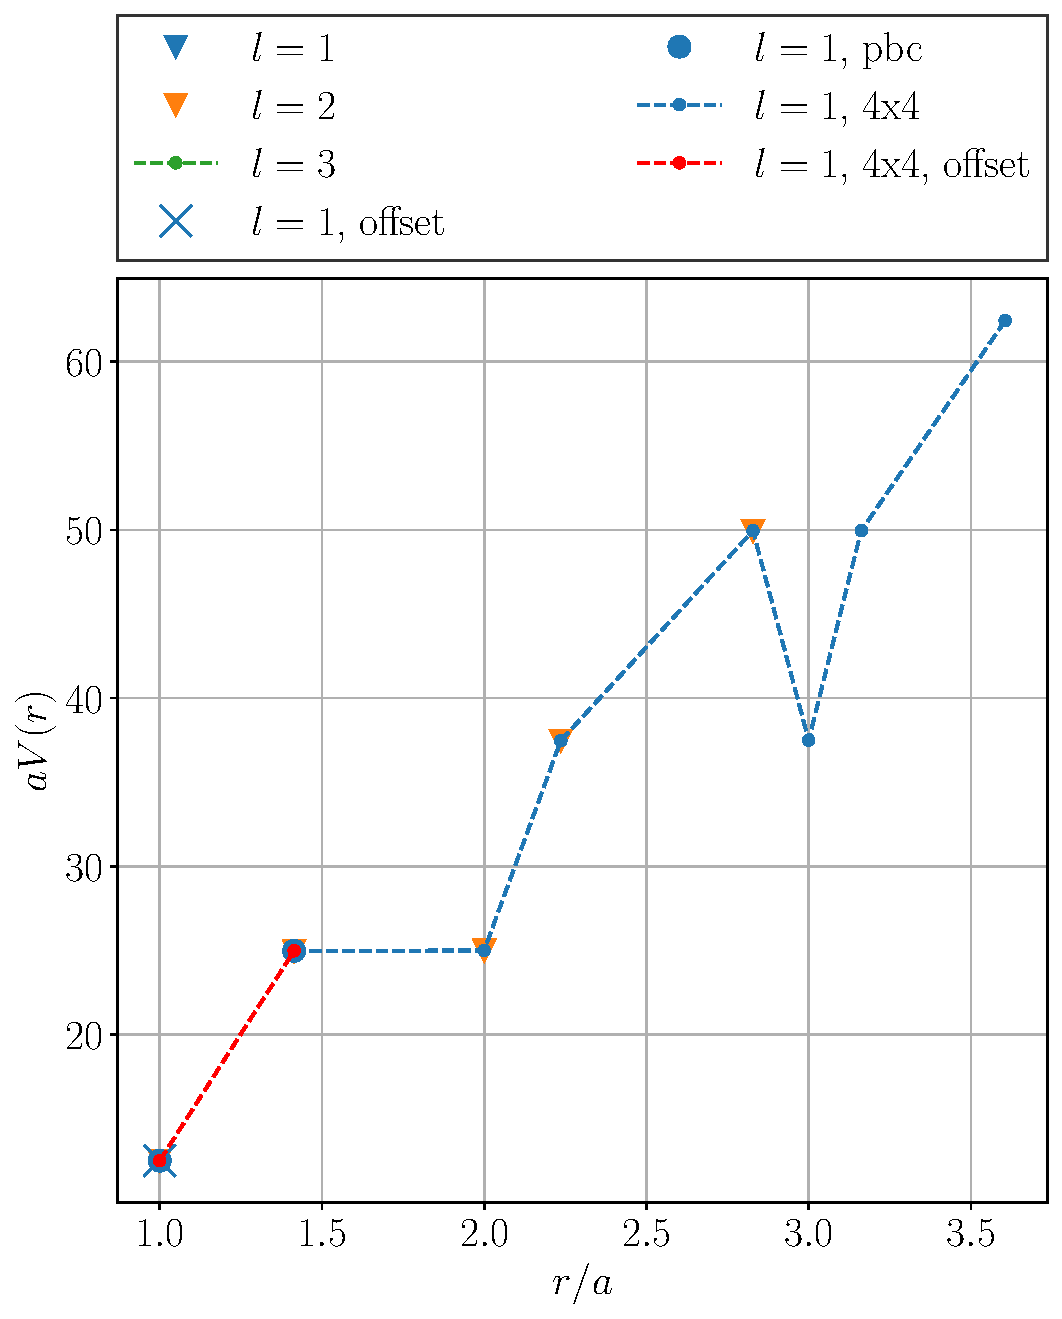
\includegraphics[width=0.45\textwidth]{images/quark_antiquark_potential_g_5.pdf}
	\end{center}
	\caption{Quark-Antiquark potential at $g=\num{5}$. By default $3\cross3$ dimensions and no PBC, if not stated otherwise.}\label{fig:qqbarl}
\end{figure}
The linearity of the potential starts to vanish and instead steps emerge, which shows that for strong coupling the lattice fragments are intensified.
There is no separation between the different setups. This is due to the fact, that at this strong coupling regime the theory starts to break down and very weak truncation or large lattices are needed, to be significant.% TODO: more
After strong couplings, weak couplings are now considered. The coupling $g=0.5$ is computed with the results in \Cref{fig:qqbars5}.
\begin{figure}[h]
	\begin{center}
		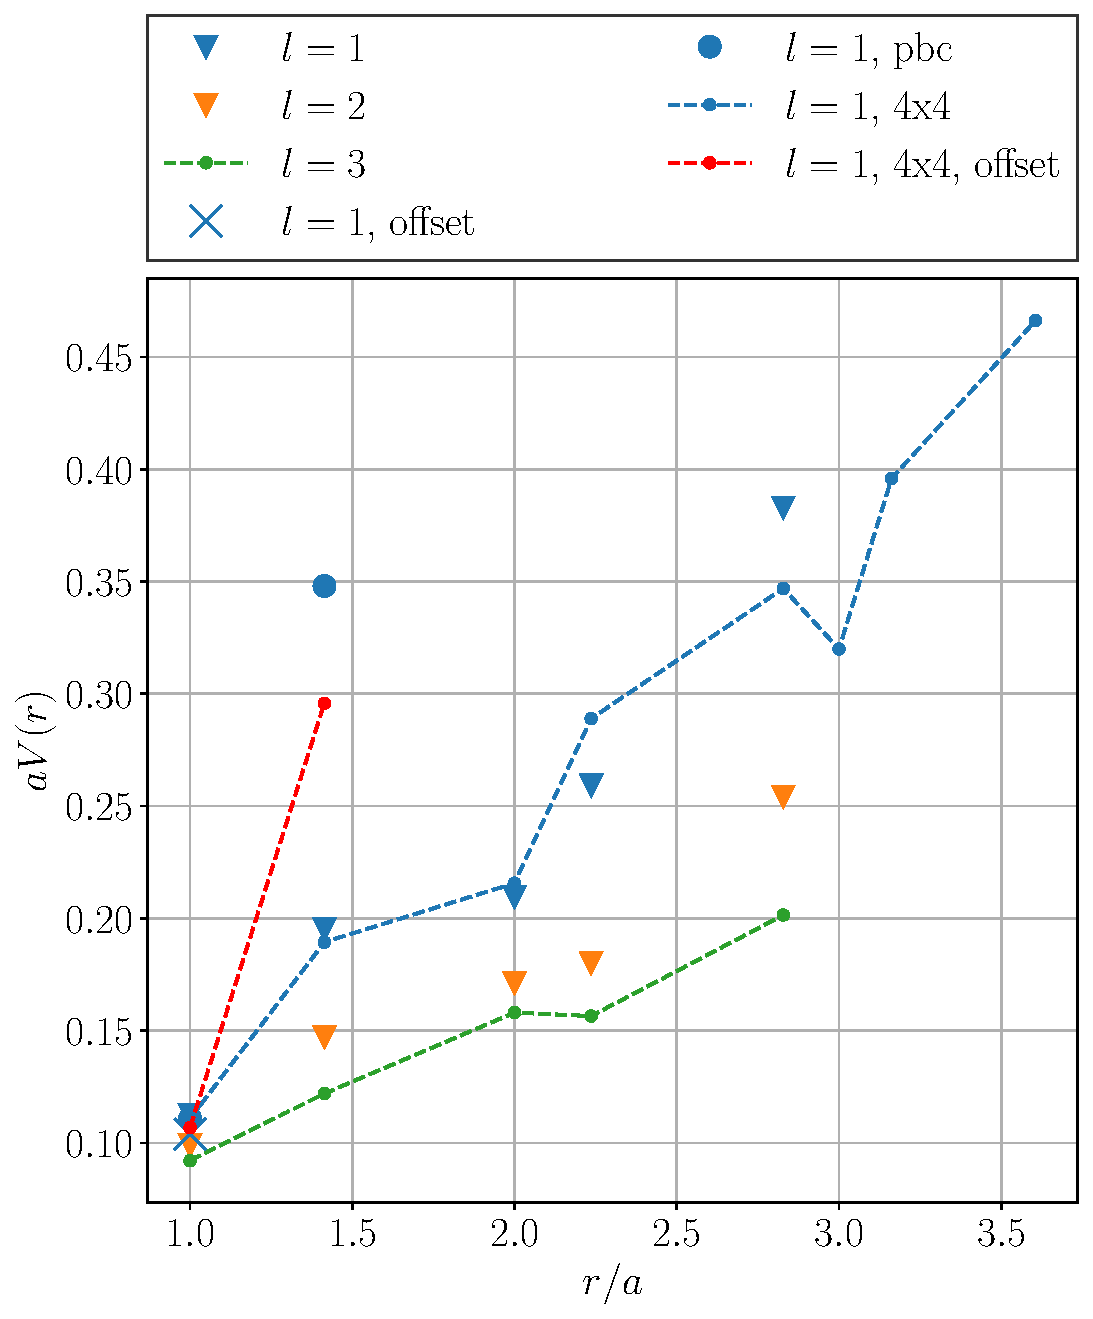
\includegraphics[width=0.45\textwidth]{images/quark_antiquark_potential_g_0.5.pdf}
	\end{center}
	\caption{Quark-Antiquark potential for different but comparable setups at $g=\num{0.5}$. By default $3\cross3$ dimensions and no PBC, if not stated otherwise.}\label{fig:qqbars5}
\end{figure}
A large separation of the potentials is seen, which shows that this coupling is in appropriate regime for this lattice, such that the approach to continuity is relevant.

With decreasing the coupling even more to $g=0.1$, \Cref{fig:qqbars1} is obtained.
\begin{figure}[h]
	\begin{center}
		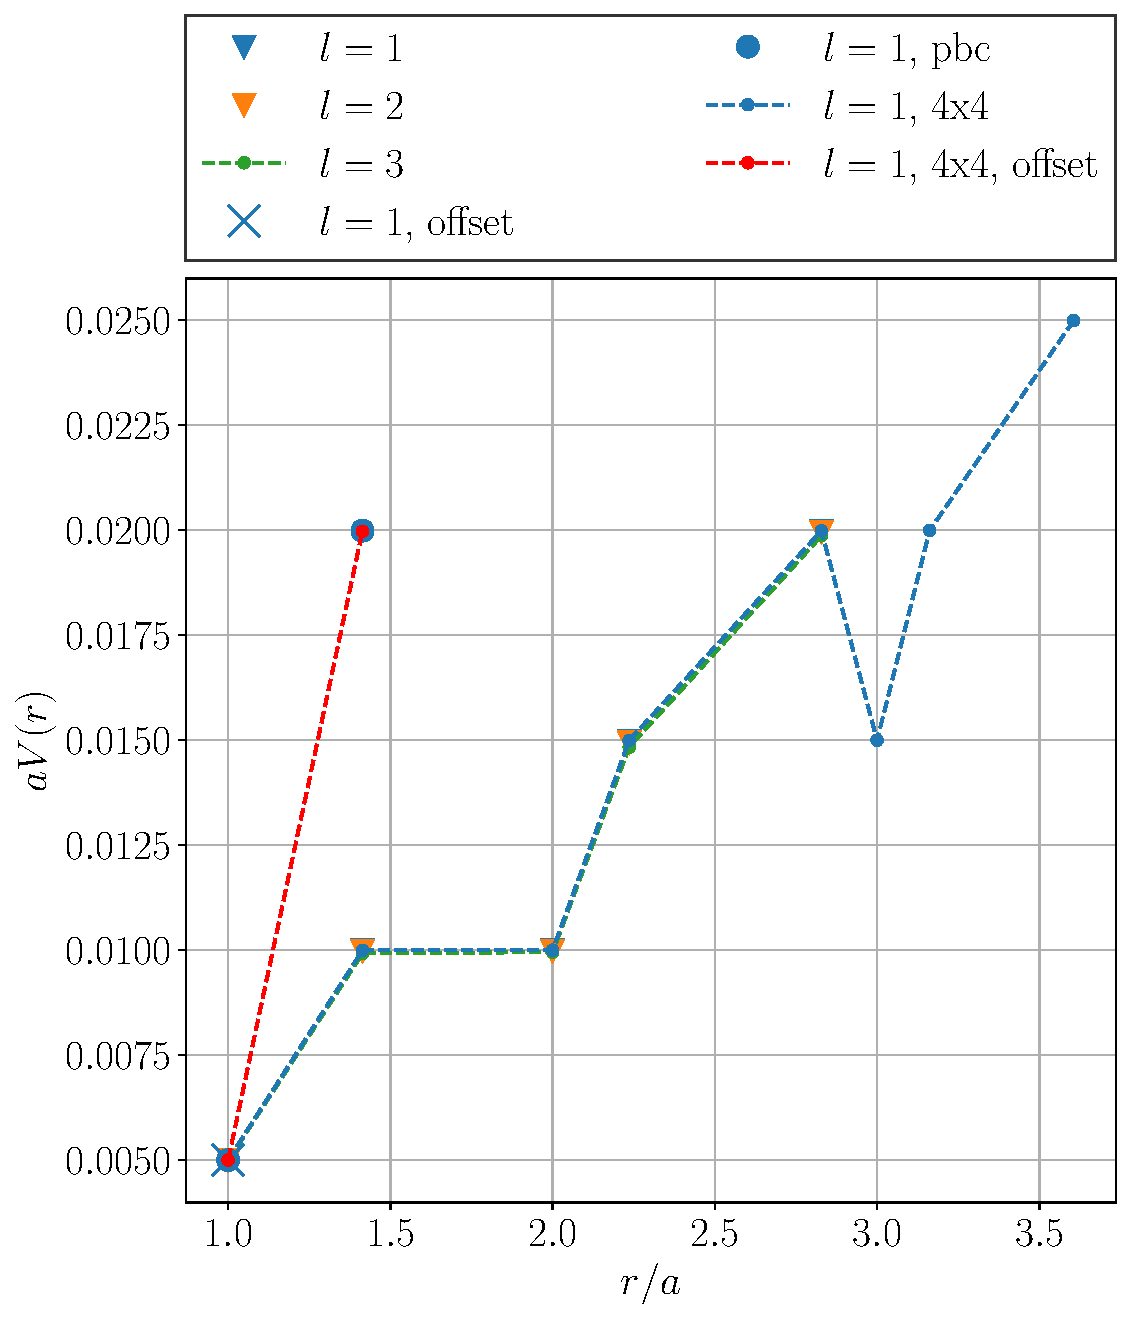
\includegraphics[width=0.45\textwidth]{images/quark_antiquark_potential_g_0.1.pdf}
	\end{center}
	\caption{Quark-Antiquark potential for different but comparable setups at $g=\num{0.1}$. By default $3\cross3$ dimensions and no PBC, if not stated otherwise.}\label{fig:qqbars1}
\end{figure}
Here a coupling regime is reached, where the lattice size fails to describe the continuum theory not even in a approximation. Neither the weakening in truncation to $l=2$ or $l=3$, nor the centering is relevant. Only the $4\cross4$ with offset and the PBC lattice show the capability to be somewhat usable, to approach continuum theory.


% TODO: A $3\cross3$ lattice with $l=2$ and PBC has \num{1.9e6} physical states and takes about an hour. A $5\cross 5$ lattice with $l=1$ and no PBC has \num{}


\iffalse
	\subsection{Step scaling}
	\begin{figure}[h]
		\begin{center}
			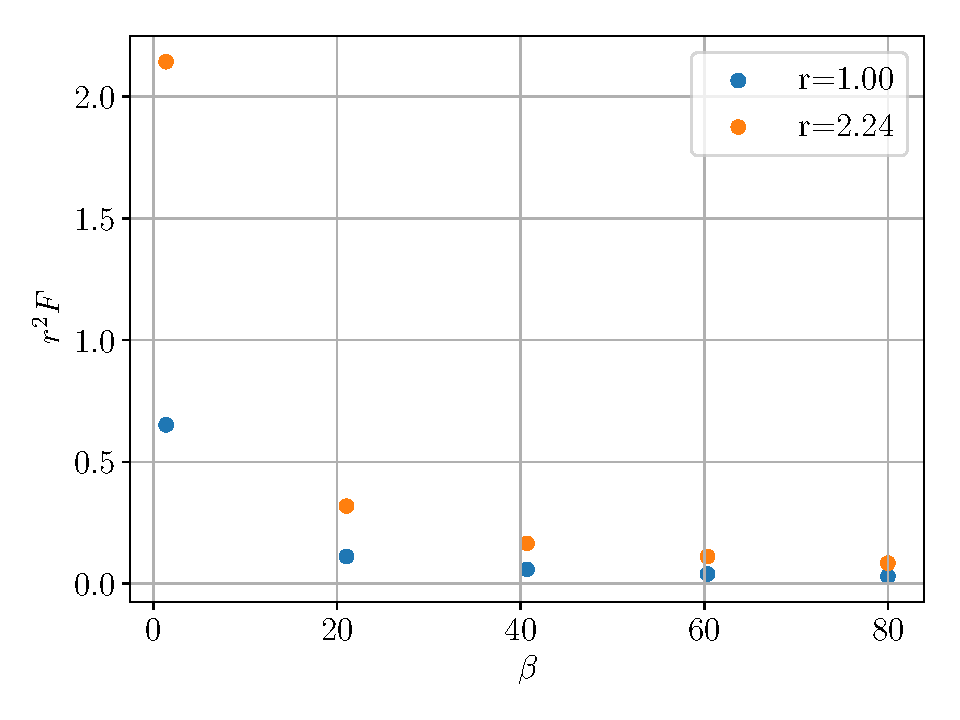
\includegraphics[width=0.45\textwidth]{images/step_scaling.pdf}
		\end{center}
		\caption{Step scaling}
	\end{figure}
\fi
